\documentclass[
    table,
    12pt,
    oneside, % symmetric pagination
    a4paper,
    %english,
    italian
]{book}

\PassOptionsToPackage{dvipsnames}{xcolor} % colori PDF/A

\usepackage{colorprofiles}
% PDF/A
% validate in https://www.pdf-online.com/osa/validate.aspx
\usepackage[a-1a,mathxmp]{pdfx}[2018/12/22]
%\usepackage{amsmath,amssymb,amsthm} % matematica
\usepackage[T1]{fontenc}
\usepackage[utf8]{inputenc}
\usepackage[italian]{babel}
\usepackage{bookmark}
\usepackage{caption}
\usepackage{chngpage, calc} % centra il frontespizio
\usepackage{csquotes} % gestisce automaticamente i caratteri (")
\usepackage{emptypage} % pagine vuote senza testatina e piede di pagina
\usepackage{epigraph} % per epigrafi
\usepackage{indentfirst} % rientra il primo paragrafo di ogni sezione
\usepackage{graphicx} % immagini
\usepackage[pdfa]{hyperref} % collegamenti ipertestuali
\usepackage{listings} % codici
%\usepackage{microtype} % microtipografia
\usepackage{mparhack,relsize}  % finezze tipografiche
\usepackage{nameref} % visualizza nome dei riferimenti
\usepackage[font=small]{quoting} % citazioni
\usepackage{subfig} % sottofigure, sottotabelle
\usepackage[italian]{varioref} % riferimenti completi della pagina
%\usepackage{booktabs} % tabelle
%\usepackage{tabularx} % tabelle di larghezza prefissata
\usepackage{longtable} % tabelle su più pagine
%\usepackage{ltxtable} % tabelle su più pagine e adattabili in larghezza
\usepackage[toc, acronym, automake]{glossaries}
\usepackage{lmodern}
\usepackage[top=3cm, bottom=2.75cm, right=3cm, left=3.75cm]{geometry} % 1in+17pt+0.6cm
\usepackage{fancyhdr}
\usepackage{lipsum}
\usepackage{setspace}
\usepackage{titlesec}
\usepackage[backend=biber,style=verbose-ibid,hyperref,backref, style=numeric, defernumbers=true]{biblatex} 
% Load variables
\newcommand{\myUni}{Università degli Studi di Padova}
\newcommand{\myDepartment}{Dipartimento di Matematica ``Tullio Levi-Civita''}
\newcommand{\myFaculty}{Corso di Laurea in Informatica}
\newcommand{\myTitle}{Test Automatici con Large Language Model}
\newcommand{\myDegree}{Tesi di Laurea Triennale}
\newcommand{\profTitle}{Prof.}
\newcommand{\myProf}{Ballan Lamberto}
\newcommand{\graduateTitle}{Laureando}
\newcommand{\myName}{Dugo Alberto}
\newcommand{\myStudentID}{2042382}
\newcommand{\myAA}{2023-2024}
\newcommand{\myLocation}{Padova}
\newcommand{\myTime}{Luglio 2024}
% Acronyms
\newacronym[description={\glslink{llmg}{Large Language Model}}]{llm}{LLM}{Large Language Model}
\newacronym[description={\glslink{ideg}{Integrated Development Environment}}]{ide}{IDE}{Integrated Development Environment}
\newacronym[description={\glslink{LoRAg}{Low-Rank Adaptation}}]{lora}{LoRA}{Low-Rank Adaptation}
\newacronym[description={\glslink{llmse}{Assured LLM-Based Software Engineering}}]{llmse}{LLMSE}{Assured LLM-Based Software Engineering}
\newacronym[description={\glslink{peft}{Parameter Efficient Fine-Tuning}}]{peft}{PEFT}{Parameter Efficient Fine-Tuning}
% Glossary
\newglossaryentry{llmg}{
    name=\glslink{llm}{LLM},
    text={Large Language Model},
    sort=llm,
    description={Un Large Language Model (LLM) è un modello capace di generare testi in linguaggio naturale basandosi su modelli statistici.
    Questi modelli acquisiscono una conoscenza linguistica attraverso l'apprendimento di relazioni statistiche durante un processo di addestramento computazionalmente oneroso.}
}

\newglossaryentry{ideg}{
    name=\glslink{ide}{IDE},
    text={Integrated Development Environment},
    sort=ide,
    description={Un Integrated Development Environment (IDE) è un'applicazione software che fornisce servizi per facilitare lo sviluppo di software. Un IDE generalmente comprende un editor di codice sorgente, strumenti di compilazione e debugging e un ambiente per eseguire il software in sviluppo.}
}

\newglossaryentry{LoRAg}{
    name=\glslink{lora}{LoRA},,
    text={Low-Rank Adaptation},
    sort=LoRA,
    description={Approccio di \gls{fine-tuning} il quale permette di costruire diversi modelli per \textit{downstream tasks} i quali ne condividono uno pre-addestrato.}
}

\newglossaryentry{fine-tuning}{
    name={Fine-tuning},
    text={fine-tuning},
    sort=fine-tuning,
    description={Metodologia che permette, attraverso modifiche minimali agli iperparametri di una \textit{neural network}, di adattare un modello ad un nuovo dataset senza doverlo riaddestrare, ottenendo quindi un modello più accurato.}
}

\newglossaryentry{mclearning}{
    name={Machine learning},
    text={machine learning},
    sort=Machine learning,
    description={Branca dell'\textit{intelligenza artificiale} che utilizza metodi statistici per migliorare la performance di un algoritmo nell'identificare pattern nei dati, imparando da questi a svolgere delle funzioni piuttosto che attraverso la programmazione esplicita.}
}

\newglossaryentry{prototipog}{
    name={Prototipo},
    text={prototipo},
    sort=prototipo,
    description={Un prototipo è un esemplare o un modello di un prodotto o di un sistema che viene realizzato antecedentemente al prodotto finale}
}

\newglossaryentry{deeplearning}{
    name={Deep learning},
    text={deep learning},
    sort=Deep learning,
    description={ADD DESCRIPTION.}
}

\newglossaryentry{llmseg}{
    name={Assured LLM-Based Software Engineering},
    text={Assured LLM-Based Software Engineering},
    sort=assured LLM-Based Software Engineering,
    description={ADD DESCRIPTION.}
}
\newglossaryentry{peftg}{
    name={Parameter Efficient Fine-Tuning},
    text={Parameter Efficient Fine-Tuning},
    sort=parameter Efficient Fine-Tuning,
    description={ADD DESCRIPTION.}
}

% Define custom colors
\definecolor{hyperColor}{HTML}{930000}
\definecolor{tableGray}{HTML}{F5F5F7}

% Set line height
\linespread{1.5}

% Custom hyphenation rules
\hyphenation {
    e-sem-pio
    ex-am-ple
}

% Images path
\graphicspath{{img/}}

% Force page color, as some editors set a grayish color as default
\pagecolor{white}

% Better spacing for footnotes
\setlength{\skip\footins}{5mm}
\setlength{\footnotesep}{5mm}

\setlength{\headheight}{14.5pt}
\addtolength{\topmargin}{-2.45pt}

% Listings setup
\lstset{
    language=[LaTeX]Tex,%C++,
    keywordstyle=\color{RoyalBlue}, %\bfseries,
    basicstyle=\small\ttfamily,
    %identifierstyle=\color{NavyBlue},
    commentstyle=\color{Green}\ttfamily,
    stringstyle=\rmfamily,
    numbers=none, %left,%
    numberstyle=\scriptsize, %\tiny
    stepnumber=5,
    numbersep=8pt,
    showstringspaces=false,
    breaklines=true,
    frameround=ftff,
    frame=single
}

% Add a subscript G to a glossary entry
\newcommand{\glox}{\textsubscript{\textbf{\textit{G }}}}

% If the subscript G is followed by a punctuation character, or anything else, you need to use \gloxspacing to prevent rendering issues, where the characters collide. Example in Chapter 7
\newcommand{\gloxspacing}{\hspace{-0.3em}}

% Improvements the paragraph command
\titleformat{\paragraph}
{\normalfont\normalsize\bfseries}{\theparagraph}{1em}{}
\titlespacing*{\paragraph}
{0pt}{3.25ex plus 1ex minus .2ex}{1.5ex plus .2ex}

% Define use case environment
\newcounter{usecasecounter} % define a counter
\setcounter{usecasecounter}{0} % set the counter to some initial value
% Parameters
% #1: ID
% #2: Nome
\newenvironment{usecase}[2]{
    \renewcommand{\theusecasecounter}{\usecasename #1}  % this is where the display of the counter is overwritten/modified
    \refstepcounter{usecasecounter} % increment counter
    \vspace{2em}
    \par \noindent % start new paragraph
    {\normalsize \textbf{\usecasename #1: #2}} % display the title before the content of the environment is displayed
    \vspace{.5em}
}{
    \medskip
}
\newcommand{\usecasename}{UC}
\newcommand{\usecaseactors}[1]{\textbf{\\Attori Principali:} #1}
\newcommand{\usecasepre}[1]{\textbf{\\Precondizioni:} #1}
\newcommand{\usecasedesc}[1]{\textbf{\\Descrizione:} #1}
\newcommand{\usecasepost}[1]{\textbf{\\Postcondizioni:} #1}
\newcommand{\usecasealt}[1]{\textbf{\\Scenario Alternativo:} #1}

% Define risks environment
\newcounter{riskcounter} % define a counter
\setcounter{riskcounter}{0} % set the counter to some initial value
% Parameters
% #1: Title
\newenvironment{risk}[1]{
    \refstepcounter{riskcounter} % increment counter
    \par \noindent % start new paragraph
    \textbf{\arabic{riskcounter}. #1} % display the title before the content of the environment is displayed
}{
    \par\medskip
}
\newcommand{\riskname}{Rischio}
\newcommand{\riskdescription}[1]{\textbf{\\Descrizione:} #1.}
\newcommand{\risksolution}[1]{\textbf{\\Soluzione:} #1.}

% Apply fancy styling to pages
\pagestyle{fancy}
\fancyhf{}
\fancyhead[L]{\leftmark} % Places Chapter N. Chatper title on the top left
\fancyfoot[C]{\thepage} % Page number in the center of the footer

% Adds a blank page while increasing the page number
\newcommand\blankpage{ 
    \clearpage
    \begingroup
      \null
      \thispagestyle{empty}
      \hypersetup{pageanchor=false}
      \clearpage
    \endgroup
}

% Increase page numbering
\newcommand\increasepagenumbering{
    \addtocounter{page}{+1}
}

% Make glossaries and bibliography
\makeglossaries
\bibliography{references/bibliography}
\defbibheading{bibliography} {
    \cleardoublepage
    \phantomsection
    \addcontentsline{toc}{chapter}{\bibname}
    \chapter*{\bibname\markboth{\bibname}{\bibname}}
}
\glsaddall

% Set up hyperlinks
\hypersetup{
    colorlinks=true,
    linktocpage=true,
    pdfstartpage=1,
    pdfstartview=,
    breaklinks=true,
    pdfpagemode=UseNone,
    pageanchor=true,
    pdfpagemode=UseOutlines,
    plainpages=false,
    bookmarksnumbered,
    bookmarksopen=true,
    bookmarksopenlevel=1,
    hypertexnames=true,
    pdfhighlight=/O,
    allcolors = hyperColor
}

% Set up captions
\captionsetup{
    tableposition=top,
    figureposition=bottom,
    font=small,
    format=hang,
    labelfont=bf
}

\date{}

\hypersetup{pdfstartview=}
\begin{document}
    %\layout
    \frontmatter
    \begin{titlepage}
    \begin{center}
        \begin{Large}
            \textbf{\myUni}\\
        \end{Large}

        \vspace{5pt}

        \begin{large}
            \textsc{\myDepartment}\\
        \end{large}

        \vspace{5pt}

        \begin{large}
            \textsc{\myFaculty}\\
        \end{large}

        \vspace{25pt}
        
        \begin{figure}[htbp]
            \centering
            
\includegraphics[alt={Emblema dell'Università degli Studi di Padova}, height=6cm]{img/logo_unipd.jpeg}
        \end{figure}

        
        \begin{Large}
            \textbf{\myTitle}\\
        \end{Large}

        \vspace{5pt}

        \begin{large}
            \textit{\myDegree}\\
        \end{large}

        \vspace{50pt}
        
        \begin{normalsize}
            \begin{flushleft}
                \textit{Relatore}\\
                \profTitle\ \myProf
            \end{flushleft}

            \vspace{-48pt}
            
            \begin{flushright}
                \textit{\graduateTitle}\\
                \myName\\
                Matricola \myStudentID
            \end{flushright}
        \end{normalsize}

        \vspace*{\fill}
        
        \line(1, 0){338} \\
        \begin{normalsize}
            \textsc{Anno Accademico \myAA}
        \end{normalsize}
    \end{center}
\end{titlepage}

    \increasepagenumbering % increase the page numbrering by 1, in order to cout the frontispiece
    \clearpage
\phantomsection
\thispagestyle{empty}
\hfill
\vfill

{\small\noindent\textcopyright\ \myName, \myTime. Tutti i diritti riservati. \myDegree: ``\textit{\myTitle}'', \myUni, \myDepartment.}
    \cleardoublepage
\phantomsection
\pdfbookmark{Ringraziamenti}{Ringraziamenti}

%\begin{flushright}{
    %\slshape
   %``No matter how much they want it, I want it more''} \\
    %\medskip
    %--- Lewis Hamilton
%\end{flushright}

\begingroup
\let\clearpage\relax
\let\cleardoublepage\relax
\let\cleardoublepage\relax

\chapter*{Ringraziamenti}

\noindent %Desidero esprimere la mia gratitudine al professor \myProf, mio relatore, per l'aiuto e il sostegno che mi ha dato durante la stesura dell'elaborato.

\noindent %rigraziamenti2\\
\noindent %ringraziamenti3

\vspace{0.75cm}

\noindent{\myLocation, \myTime}
\hfill \textit{\myName}

\endgroup

    \cleardoublepage
\phantomsection
\pdfbookmark{Compendio}{Compendio}
\begingroup
\let\clearpage\relax
\let\cleardoublepage\relax
\chapter*{Abstract}
Il presente documento illustra l'attività di stage svolta dal laureando Alberto Dugo presso l'azienda Zucchetti Spa.
\\Durante il periodo di stage, della durata di 320 ore, vi è stata l'opportunità di approfondire le conoscenze in ambito \gls{mclearning}\glox.
In particolare era richiesto lo studio e l'implementazione di test automatici derivanti direttamente dal codice, sfruttando le abilità dei sistemi di intelligenza artificiale ed in particolare del \gls{llm}\glox\gloxspacing.
Vi è stato inoltre la possibilità di fare \gls{fine-tuning}\glox dei modelli \gls{llm} attraverso il metodo \gls{lora}\glox e quantizzare i modelli stessi in modo da renderli più efficienti.
\endgroup
\vfill

    \blankpage % example of a blank page, that also increases the page couter by 1
    \cleardoublepage
\pdfbookmark{\contentsname}{tableofcontents}
\setcounter{secnumdepth}{5}  % Numbering depth for sections
\setcounter{tocdepth}{5}     
% Depth of entries in the table of contents

\tableofcontents
%\markboth{\contentsname}{\contentsname}
\clearpage

\begingroup
    \let\clearpage\relax
    \let\cleardoublepage\relax
    \let\cleardoublepage\relax

    % Figures list
    \phantomsection
    \pdfbookmark{\listfigurename}{lof}
    \listoffigures

    \vspace*{8ex}

    % Tables list
    \phantomsection
    \pdfbookmark{\listtablename}{lot}
    \listoftables

    \vspace*{8ex}
\endgroup

\cleardoublepage
    

    \mainmatter
    \chapter{Introduzione}
\label{chap:introduzione}



%Introduzione al contesto applicativo.

%Lorem Figure \ref{fig:entanglement}

%Esempio di utilizzo di un termine nel glossario \gls{api}.

%Esempio di citazione nel piè di pagina citazione\footcite{womak:lean-thinking}

%\lipsum[1-2]

\section{L'azienda}
\begin{figure}[h!]
    \centering
    
\includegraphics[alt={Testo alternativo dell'immagine}, width=0.7\columnwidth]{img/logoZucchetti.jpeg}
    \caption{logo di Zucchetti}
    \label{fig:entanglement}
\end{figure}
Zucchetti S.p.a. è la prima software house in Italia per fatturato, opera nel settore dell'\textit{Information Technology}, ed è stata fondata nel 1978 da Fabrizio Bernini a Lodi. 
L'azienda è specializzata nella realizzazione di software gestionali per pianificazione delle risorse d'impresa, soluzioni per il controllo degli accessi e sistemi di automazione industriale. 
Al giorno d'oggi Zucchetti oltre ad avere sedi in tutta Italia è presente anche in 50 paesi esteri, tra cui Cina, Germania, USA e Svizzera e conta più di 8.000 dipendenti e più di 1650 \textit{partner}.

\section{Il progetto}
Lo \textit{stage} si è svolto presso l'azienda Zucchetti, con sede a Padova. Il progetto di \textit{stage} ha previsto la ricerca e lo sviluppo di test automatici derivanti direttamente dal codice e dalla documentazione, sfruttando le abilità dei sistemi di \textit{intelligenza artificiale} ed in particolare dei \glspl{llmg}.
Lo \textit{stage} è stato diviso in due macroperiodi di quattro settimane ciascuno. Nel primo periodo ho analizzato, attraverso lo studio di paper accademici e documentazioni, le tecniche di \textit{testing} che sfruttano \glspl{llmg}. Successivamente ho implementato un \gls{prototipog} di generatore di test automatici in \textit{Python} che usufruisce di un modello basato su \textit{natural language processing}. Nella seconda parte del primo periodo ho decorato il codice attraverso commenti e ho generato \textit{test}. I risultati di questi sono stati poi confrontati con quelli ottenuti dalla prima parte di periodo. Nel secondo periodo invece ho eseguito \gls{fine-tuning} dei modelli \glspl{llm} con il metodo \gls{lora}, per poi confrontare i risultati ottenuti con quelli nel primo periodo.
È stato inoltre richiesto lo studio di tecniche di \textit{quantizzazione} per ridurre la dimensione dei modelli \glspl{llm} e la loro complessità computazionale.
\section{Organizzazione del testo}
\begin{description}
    \item[{\hyperref[chap:processi-metodologie]{Il secondo capitolo}}] descrive i processi e le metodologie utilizzate durante lo \textit{stage}. In particolare si approfondiranno i processi di sviluppo \textit{software} e gli strumenti utilizzati per fare ciò.
    
    \item[{\hyperref[chap:descrizione-stage-1]{Il terzo capitolo}}] si propone di delineare il dominio applicativo del progetto, mediante un'analisi dettagliata del tema accompagnata da esempi pratici di utilizzo. 
    Inoltre, si provvederà a fornire una descrizione esaustiva del funzionamento di \textit{Assured LLMS}. 
    In questa sezione, sarà altresì redatta una lista esaustiva di rischi, requisiti e obiettivi del progetto. 
    Successivamente, si procederà con la descrizione del prodotto sviluppato, che includerà \textit{script} e \textit{benchmarks}. 

    \item[{\hyperref[chap:descrizione-stage-2]{Il quarto capitolo}}] descrive il processo di applicazione di \gls{lora} e le possibili ottimizzazioni, andando ad approfondire le tecniche utilizzate durante il processo.

    \item[{\hyperref[chap:conclusioni]{Il quinto capitolo}}] concluderà il documento, presentando una valutazione retrospettiva personale dell'esperienza di \textit{stage} e delle conoscenze acquisite.
    
\end{description}

In seguito si possono trovare le convenzioni tipografiche utilizzate per la stesura del documento:
\begin{itemize}
	\item gli acronimi, le abbreviazioni e i termini ambigui o di uso non comune menzionati vengono definiti nel glossario, situato alla fine del presente documento;
	\item per la prima occorrenza dei termini riportati nel glossario viene utilizzata la seguente nomenclatura: \textit{parola}\glox\gloxspacing;
	\item i termini in lingua straniera o facenti parti del gergo tecnico sono evidenziati con il carattere \textit{corsivo}.
\end{itemize}

\newpage
    \chapter{Processi e metodologie}
\label{chap:processi-metodologie}

Lorem ipsum dolor sit amet, consectetuer adipiscing elit. Aenean commodo ligula eget dolor. Aenean massa. Cum sociis natoque\footnote{\cite{site:agile-manifesto}} penatibus et magnis dis parturient montes, nascetur ridiculus mus. Donec quam felis, ultricies nec\footnote{\cite{article:spooky}}, pellentesque eu, pretium quis, sem.

\begin{figure}[h]
    \centering
    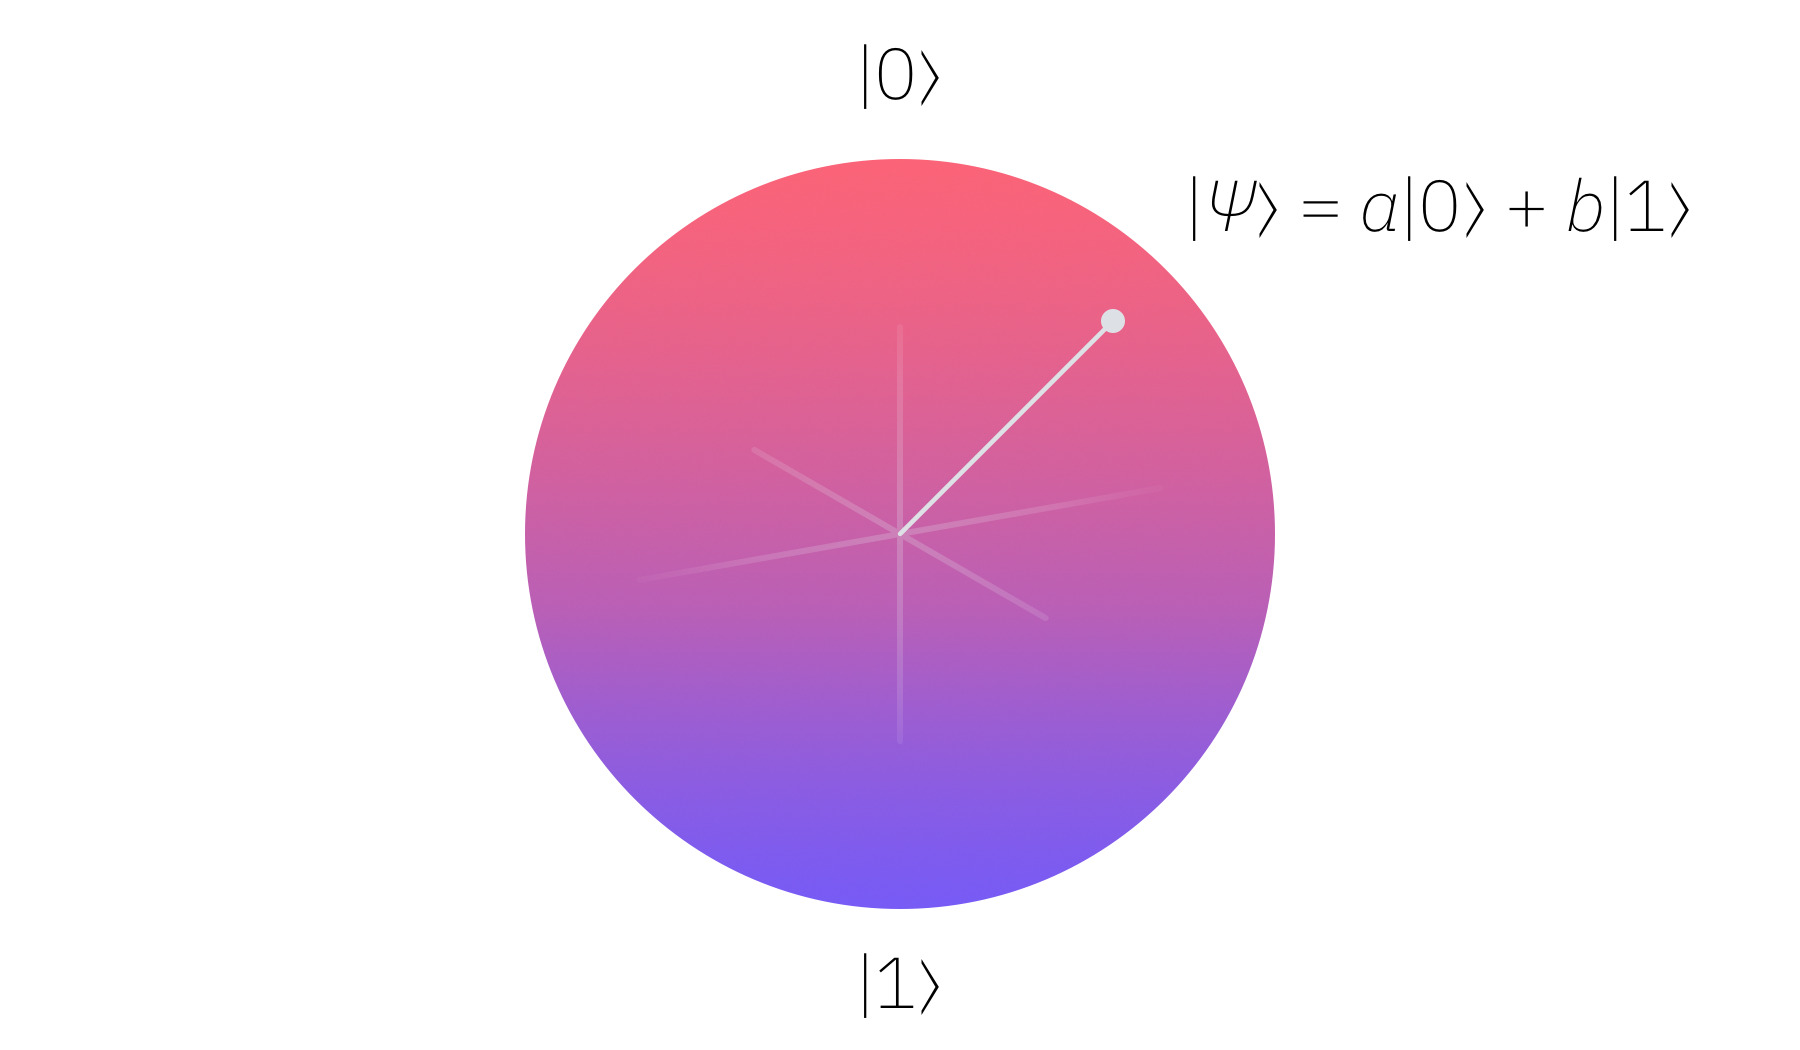
\includegraphics[alt={Testo alternativo dell'immagine}, height=5cm]{img/qubit.jpeg}
    \caption{Lorem}
    \label{fig:qubit}
\end{figure}
\lipsum[1]

\section{Processo sviluppo prodotto}
\lipsum[1-2]

\newpage
    \chapter{Descrizione dello stage}
\label{chap:descrizione-stage}

\section{Introduzione al progetto}
\begin{figure}[!ht] 
    \centering 
    
\includegraphics[alt={Testo alternativo dell'immagine}, width=0.5\columnwidth]{img/pk_estate.jpeg}
    \caption{Caption}
    \label{fig:pk_estate}
\end{figure}
\lipsum[1]

\section{Analisi preventiva dei rischi}

Durante la fase di analisi iniziale sono stati individuati alcuni possibili rischi a cui si potrà andare incontro.
Si è quindi proceduto a elaborare delle possibili soluzioni per far fronte a tali rischi.

\begin{risk}{Performance del simulatore hardware}
    \riskdescription{le performance del simulatore hardware e la comunicazione con questo potrebbero risultare lenti o non abbastanza buoni da causare il fallimento dei test}
    \risksolution{coinvolgimento del responsabile a capo del progetto relativo il simulatore hardware}
    \label{risk:hardware-simulator} 
\end{risk}

\section{Requisiti e obiettivi}

\begin{center}
    \rowcolors{1}{}{tableGray}
    \begin{longtable}{|p{2.25cm}|p{7.75cm}|p{2.25cm}|}
    \hline
    \multicolumn{1}{|c|}{\textbf{A}} & \multicolumn{1}{c|}{\textbf{B}}\\ 
    \hline 
    \endfirsthead
    \multicolumn{3}{c}%
    {{\bfseries \tablename\ \thetable{} -- Continuo della tabella}}\\
    \hline
    \multicolumn{1}{|c|}{\textbf{A}} & \multicolumn{1}{c|}{B}\\ \hline 
    \endhead
    \hline
    \multicolumn{3}{|r|}{{Continua nella prossima pagina...}}\\
    \hline
    \endfoot
    \endlastfoot 
    
    AA & BB \\
    \hline
    AA & BB \\
    \hline
    AA & BB \\
    \hline
    AA & BB \\
    \hline
    \hiderowcolors
    \caption{Lorem.}
    \label{tab:requisiti_obbiettivi}
    \end{longtable}
\end{center}

\section{Pianificazione}
\begin{figure}[!ht] 
    \centering 
    
\includegraphics[alt={Testo alternativo dell'immagine}, width=0.5\columnwidth]{img/pk_estate.jpeg}
    \caption{Caption}
    \label{fig:pk_estate_2}
\end{figure}
\lipsum[1]

\subsection{subsection}
\lipsum[1]

\subsubsection{subsubsection}
\lipsum[1]

\paragraph{paragraph}
\lipsum[1]

\newpage
    \chapter{Analisi dei requisiti}
\label{chap:analisi-requisiti}

\section{Casi d'uso}
Per lo studio dei casi di utilizzo del prodotto sono stati creati dei diagrammi.
I diagrammi dei casi d'uso (in inglese \textit{Use Case Diagram}) sono diagrammi di tipo \gls{uml} dedicati alla descrizione delle funzioni o servizi offerti da un sistema, così come sono percepiti e utilizzati dagli attori che interagiscono col sistema stesso.
Essendo il progetto finalizzato alla creazione di un tool per l'automazione di un processo, le interazioni da parte dell'utilizzatore devono essere ovviamente ridotte allo stretto necessario. Per questo motivo i diagrammi d'uso risultano semplici e in numero ridotto.

\begin{figure}[ht]
    \vspace{2em}
    \centering
    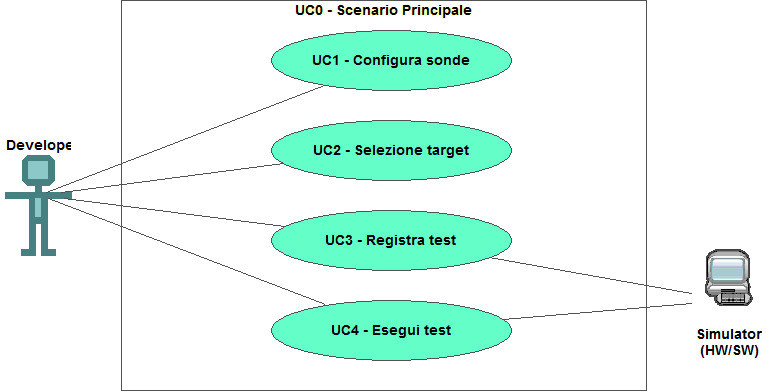
\includegraphics[alt={Testo alternativo dell'immagine}, width=0.75\columnwidth]{img/usecase/scenario-principale.jpeg}
    \caption{Use Case 0: Scenario principale}
    \label{fig:scenario_principale}
\end{figure}

\begin{usecase}{0}{Scenario principale}
    \usecaseactors{Sviluppatore applicativi.}
    \usecasepre{Lo sviluppatore è entrato nel plugin di simulazione all'interno dell'IDE.}
    \usecasedesc{La finestra di simulazione mette a disposizione i comandi per configurare, registrare o eseguire un test.}
    \usecasepost{Il sistema è pronto per permettere una nuova interazione.}
    \label{uc:uc_scenario_principale}
\end{usecase}

\begin{usecase}{1}{Gestione Utente}
    \usecaseactors{Amministratore, Utente Registrato.}
    \usecasepre{L'utente deve essere autenticato nel sistema.}
    \usecasedesc{L'utente può gestire le informazioni del proprio profilo.}
    \usecasepost{Le modifiche vengono salvate nel sistema.}
    \usecasealt{Se l'utente non è autenticato, visualizza un messaggio di errore.}
    \label{uc:uc_casi_uso}
\end{usecase}

\begin{usecase}{2}{Creazione Prodotto}
    \usecaseactors{Amministratore.}
    \usecasepre{L'amministratore ha effettuato l'accesso al sistema.}
    \usecasedesc{L'amministratore può aggiungere un nuovo prodotto al catalogo.}
    \usecasepost{Il nuovo prodotto viene aggiunto con successo.}
    \usecasealt{Se i campi obbligatori non sono compilati, visualizza un messaggio di errore.}
    \label{uc:uc_creazione_prodotto}
\end{usecase}

\section{Tracciamento dei requisiti}
Da un'attenta analisi dei requisiti e degli use case effettuata sul progetto è stata stilata la tabella che traccia i requisiti in rapporto agli use case.\\
Sono stati individuati diversi tipi di requisiti e si è quindi fatto utilizzo di un codice identificativo per distinguerli.\\
Il codice dei requisiti, dove ogni requisito è identificato con il carattere \textbf{R}, è così strutturato:
\begin{enumerate}
    \item[\textbf{F}:] Funzionale.
    \item[\textbf{Q}:] Qualitativo.
    \item[\textbf{V}:] Di vincolo.
    \item[\textbf{N}:] Obbligatorio (necessario).
    \item[\textbf{D}:] Desiderabile.
    \item[\textbf{Z}:] Opzionale.
\end{enumerate}

Nelle tabelle \ref{tab:requisiti_funzionali}, \ref{tab:requisiti_qualitativi} e \ref{tab:requisiti_vincolo} sono riassunti i requisiti e il loro tracciamento con gli use case delineati in fase di analisi.

\section{Tabelle dei requisiti}
\begin{center}
    \rowcolors{1}{}{tableGray}
    \begin{longtable}{|p{2.25cm}|p{7.75cm}|p{2.25cm}|}
    \hline 
    \multicolumn{1}{|c|}{\textbf{Requisito}} & \multicolumn{1}{c|}{\textbf{Descrizione}} & \multicolumn{1}{c|}{\textbf{Use Case}}\\
    \hline 
    \endfirsthead
    \multicolumn{3}{c}
    {{\bfseries \tablename\ \thetable{} -- Continuo della tabella}}\\
    \hline
    \multicolumn{1}{|c|}{\textbf{Requisito}} & \multicolumn{1}{c|}{\textbf{Descrizione}} & \multicolumn{1}{c|}{\textbf{Use Case}}\\
    \hline 
    \endhead
    \hline
    \multicolumn{3}{|r|}{{Continua nella prossima pagina...}} \\ \hline
    \endfoot
    \endlastfoot
    
    RFN-1 & L’interfaccia permette di configurare il tipo di sonde del test & UC1 \\
    \hline
    \hiderowcolors
    \caption{Tabella del tracciamento dei requisiti funzionali.}
    \label{tab:requisiti_funzionali}
    \end{longtable}
\end{center}

\begin{center}
    \rowcolors{1}{}{tableGray}
    \begin{longtable}{|p{2.25cm}|p{7.75cm}|p{2.25cm}|}
    \hline 
    \multicolumn{1}{|c|}{\textbf{Requisito}} & \multicolumn{1}{c|}{\textbf{Descrizione}} & \multicolumn{1}{c|}{\textbf{Use Case}}\\
    \hline 
    \endfirsthead
    \multicolumn{3}{c}
    {{\bfseries \tablename\ \thetable{} -- Continuo della tabella}}\\
    \hline 
    \multicolumn{1}{|c|}{\textbf{Requisito}} & \multicolumn{1}{c|}{\textbf{Descrizione}} & \multicolumn{1}{c|}{\textbf{Use Case}}\\
    \hline 
    \endhead
    \hline 
    \multicolumn{3}{|r|}{{Continua nella prossima pagina...}}\\ 
    \hline
    \endfoot
    \endlastfoot
    
    RQD-1n & Le prestazioni del simulatore hardware deve garantire la giusta esecuzione dei test e non la generazione di falsi negativi & - \\
    \hline
    \hiderowcolors
    \caption{Tabella del tracciamento dei requisiti qualitativi.}
    \label{tab:requisiti_qualitativi}
    \end{longtable}
\end{center}

\begin{center}
    \rowcolors{1}{}{tableGray}
    \begin{longtable}{|p{2.25cm}|p{7.75cm}|p{2.25cm}|}
    \hline
    \multicolumn{1}{|c|}{\textbf{Requisito}} & \multicolumn{1}{c|}{\textbf{Descrizione}} & \multicolumn{1}{c|}{\textbf{Use Case}}\\
    \hline 
    \endfirsthead
    \multicolumn{3}{c}
    {{\bfseries \tablename\ \thetable{} -- Continuo della tabella}}\\
    \hline
    \multicolumn{1}{|c|}{\textbf{Requisito}} & \multicolumn{1}{c|}{\textbf{Descrizione}} & \multicolumn{1}{c|}{\textbf{Use Case}}\\
    \hline 
    \endhead
    \hline
    \multicolumn{3}{|r|}{{Continua nella prossima pagina}}\\
    \hline
    \endfoot
    \endlastfoot
    
    RVO-1 & La libreria per l'esecuzione dei test automatici deve essere riutilizzabile & - \\
    \hline
    \hiderowcolors
    \caption{Tabella del tracciamento dei requisiti di vincolo.}
    \label{tab:requisiti_vincolo}
    \end{longtable}
\end{center}

\newpage
    \chapter{Progettazione e codifica}
\label{chap:progettazione-codifica}
Breve introduzione al capitolo

\section{Tecnologie e strumenti}
\label{sec:tecnologie-strumenti}
Di seguito viene data una panoramica delle tecnologie e strumenti utilizzati.

\subsection*{Tecnologia 1}
Descrizione Tecnologia 1.

\subsection*{Tecnologia 2}
Descrizione Tecnologia 2

\section{Ciclo di vita del software}
\label{sec:ciclo-vita-software}

\section{Progettazione}
\label{sec:progettazione}

\subsection{Namespace 1}
Descrizione namespace 1.

\section{Design Pattern utilizzati}

\section{Codifica}

\newpage
    \chapter{Verifica e validazione}
\label{chap:verifica-validazione}

\begin{figure}[h!]
    \centering
    
\includegraphics[alt={Testo alternativo dell'immagine}, width=1\columnwidth]{img/quantum_superposition.jpeg}
    \caption{Lorem}
    \label{fig:enter-label}
\end{figure}

\lipsum[1-2]

\newpage
    \chapter{Valutazione retrospettiva}
\label{chap:conclusioni}
    \section{Conoscenze acquisite}
    Durante l’esperienza in Zucchetti, sono stati affrontati diversi temi legati all'intelligenza artificiale. I \textit{test} sono stati il tema principale dello stage; infatti, sebbene le tecniche studiate fossero molto diverse tra loro, l'obiettivo principale era migliorare la generazione di \textit{test}.
    Le conoscenze acquisite sono variate notevolmente tra il primo e il secondo macro periodo. Nel primo periodo, sono state apprese nozioni riguardanti gli \gls{llmse}, che costituiscono la base del lavoro sulla generazione di \textit{test}. È stato particolarmente importante delineare un percorso per futuri approfondimenti; comprendere che i \textit{test} generati sono qualitativamente migliori se il codice è in inglese e il linguaggio è tipizzato è stato di fondamentale importanza.
    Nel secondo macro periodo, invece, le nozioni sono state principalmente legate alla specializzazione del modello tramite \gls{fine-tuning}. Sono state apprese tecniche come \gls{lora} e approfondite alcune delle possibili migliorie applicabili, come \textit{MoLE} e \textit{AdaMoLE}.
    Oltre alla specializzazione del modello, è stata esaminata a fondo la quantizzazione. Sono state approfondite le tecniche di quantizzazione asimmetrica e simmetrica e la loro applicazione agli \gls{llm}, al fine di ridurre le loro dimensioni.    
    Le conoscenze acquisite non si sono limitate all'ambito lavorativo, ma hanno arricchito anche il lato personale. Durante lo stage, sono state infatti molte le lezioni apprese, la maggior parte delle quali deriva dall'interazione con i colleghi e il responsabile dello stage, Gregorio Piccoli. Queste esperienze hanno contribuito significativamente alla crescita professionale e personale.
        %cosa ho imparato dallo stage
    \section{Valutazione personale}
            %cosa ho fatto bene -> rispetto obiettivi, integrazione col team
    La valutazione che può essere associata con l'esperienza trascorsa durante questo stage è sicuramente più che positiva.
    Durante il percorso è stato appreso come gestire un progetto in un ambiente di lavoro professionale e innovativo, ricercando efficacia, efficienza e qualità in ciò che doveva essere completato.
    È stato inoltre significativo affacciarsi al mondo della ricerca e sviluppo all'interno di una grande azienda come Zucchetti, poiché rappresenta un segmento molto interessante e dinamico. Questa esperienza ha permesso di comprendere meglio le dinamiche e le sfide legate all'innovazione tecnologica in un contesto aziendale di alto livello.
    Un'ulteriore prova del successo dello stage deriva dal rapporto personale che si è creato con i colleghi. Questo aspetto è di grande rilevanza poiché favorisce il confronto e il miglioramento delle capacità comunicative.
        %cosa avrei potuto fare meglio 
    Non vi sono solo ovviamente solo obiettivi raggiunti e rapporti instaurati, durante un primo incontro con la vita lavorativa all'interno di un'azienda sono emerse anche difficoltà. 
     La principale difficoltà è stata mantenere costanza e dedizione per raggiungere gli obiettivi prefissati, un aspetto spesso sottovalutato.
     Inoltre, sebbene il clima fosse disteso vi è stata la necessità costante di portare risultati di valore con il proprio operato, un aspetto che durante la vita universitaria spesso non si affronta.
    È importante sottolineare che sono state proprio queste piccole difficoltà che hanno accompagnato l'esperienza di stage ad accrescere l'interesse verso lo stage stesso, ponendo ogni giorno un nuovo obiettivo stimolante al fine di migliorare.

\newpage

    \pagenumbering{roman}
    \backmatter
    \chapter{Bibliografia}
\label{cap:bibliography}

\nocite{*}

% Books bibliography
\printbibliography[heading=subbibliography, title={Testi}, type=book]

% Articles bibliography
\printbibliography[heading=subbibliography, title={Articoli}, type=article]

% Websites bibliography
%\printbibliography[heading=subbibliography, title={Siti}, type=online]
    \chapter{Sitografia}
\label{cap:webliography}
\nocite{*}

% Websites bibliography
\printbibliography[heading=subbibliography, title={\null}, type=online]

    \printglossary[type=\acronymtype, title=Acronimi e abbreviazioni, toctitle=Acronimi e abbreviazioni]
    \printglossary[type=main, title=Glossario, toctitle=Glossario]
\end{document}